\documentclass{extbook}[14pt]
\usepackage{multicol, enumerate, enumitem, hyperref, color, soul, setspace, parskip, fancyhdr, amssymb, amsthm, amsmath, bbm, latexsym, units, mathtools}
\everymath{\displaystyle}
\usepackage[headsep=0.5cm,headheight=0cm, left=1 in,right= 1 in,top= 1 in,bottom= 1 in]{geometry}
\usepackage{dashrule}  % Package to use the command below to create lines between items
\newcommand{\litem}[1]{\item #1

\rule{\textwidth}{0.4pt}}
\pagestyle{fancy}
\lhead{}
\chead{Answer Key for Progress Quiz 4 Version A}
\rhead{}
\lfoot{6286-1986}
\cfoot{}
\rfoot{Fall 2020}
\begin{document}
\textbf{This key should allow you to understand why you choose the option you did (beyond just getting a question right or wrong). \href{https://xronos.clas.ufl.edu/mac1105spring2020/courseDescriptionAndMisc/Exams/LearningFromResults}{More instructions on how to use this key can be found here}.}

\textbf{If you have a suggestion to make the keys better, \href{https://forms.gle/CZkbZmPbC9XALEE88}{please fill out the short survey here}.}

\textit{Note: This key is auto-generated and may contain issues and/or errors. The keys are reviewed after each exam to ensure grading is done accurately. If there are issues (like duplicate options), they are noted in the offline gradebook. The keys are a work-in-progress to give students as many resources to improve as possible.}

\rule{\textwidth}{0.4pt}

\begin{enumerate}\litem{
Describe the end behavior of the polynomial below.
\[ f(x) = -4(x - 3)^{4}(x + 3)^{5}(x - 6)^{2}(x + 6)^{2} \]
The solution is the graph below, which is option A.
\begin{center}
    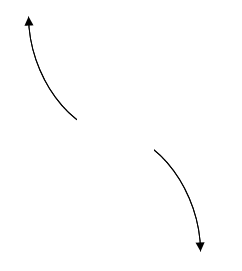
\includegraphics[width=0.3\textwidth]{../Figures/polyEndBehaviorCopyAA.png}
\end{center}\begin{enumerate}[label=\Alph*.]
\begin{multicols}{2}
\item 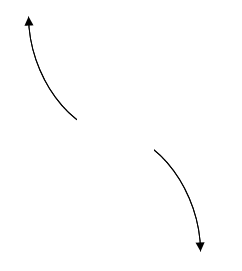
\includegraphics[width = 0.3\textwidth]{../Figures/polyEndBehaviorCopyAA.png}
\item 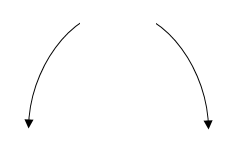
\includegraphics[width = 0.3\textwidth]{../Figures/polyEndBehaviorCopyBA.png}
\item 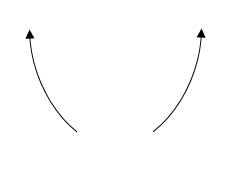
\includegraphics[width = 0.3\textwidth]{../Figures/polyEndBehaviorCopyCA.png}
\item 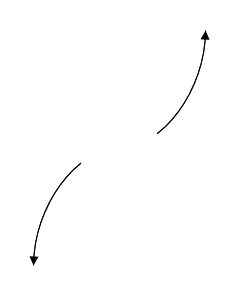
\includegraphics[width = 0.3\textwidth]{../Figures/polyEndBehaviorCopyDA.png}
\end{multicols}\item None of the above.\end{enumerate}
\textbf{General Comment:} Remember that end behavior is determined by the leading coefficient AND whether the \textbf{sum} of the multiplicities is positive or negative.
}
\litem{
Construct the lowest-degree polynomial given the zeros below. Then, choose the intervals that contain the coefficients of the polynomial in the form $ax^3+bx^2+cx+d$.
\[ -5, \frac{-3}{5}, \text{ and } \frac{6}{5} \]
The solution is \( 25x^{3} +110 x^{2} -93 x -90 \), which is option D.\begin{enumerate}[label=\Alph*.]
\item \( a \in [25, 34], b \in [106, 125], c \in [-95, -91], \text{ and } d \in [87, 95] \)

$25x^{3} +110 x^{2} -93 x + 90$, which corresponds to multiplying everything correctly except the constant term.
\item \( a \in [25, 34], b \in [-141, -137], c \in [52, 58], \text{ and } d \in [87, 95] \)

$25x^{3} -140 x^{2} +57 x + 90$, which corresponds to multiplying out $(x + 1)(5x -5)(5x -5)$.
\item \( a \in [25, 34], b \in [-112, -103], c \in [-95, -91], \text{ and } d \in [87, 95] \)

$25x^{3} -110 x^{2} -93 x + 90$, which corresponds to multiplying out $(x -5)(5x -3)(5x + 6)$.
\item \( a \in [25, 34], b \in [106, 125], c \in [-95, -91], \text{ and } d \in [-91, -88] \)

* $25x^{3} +110 x^{2} -93 x -90$, which is the correct option.
\item \( a \in [25, 34], b \in [-174, -169], c \in [239, 248], \text{ and } d \in [-91, -88] \)

$25x^{3} -170 x^{2} +243 x -90$, which corresponds to multiplying out $(x + 1)(5x + 5)(5x -5)$.
\end{enumerate}

\textbf{General Comment:} To construct the lowest-degree polynomial, you want to multiply out $(x + 5)(5x + 3)(5x -6)$
}
\litem{
Construct the lowest-degree polynomial given the zeros below. Then, choose the intervals that contain the coefficients of the polynomial in the form $x^3+bx^2+cx+d$.
\[ -2 - 3 i \text{ and } -4 \]
The solution is \( x^{3} +8 x^{2} +29 x + 52 \), which is option B.\begin{enumerate}[label=\Alph*.]
\item \( b \in [-9, -7], c \in [28.54, 29.25], \text{ and } d \in [-53, -48] \)

$x^{3} -8 x^{2} +29 x -52$, which corresponds to multiplying out $(x-(-2 - 3 i))(x-(-2 + 3 i))(x -4)$.
\item \( b \in [4, 13], c \in [28.54, 29.25], \text{ and } d \in [47, 55] \)

* $x^{3} +8 x^{2} +29 x + 52$, which is the correct option.
\item \( b \in [-7, 3], c \in [5.19, 6.76], \text{ and } d \in [3, 9] \)

$x^{3} + x^{2} +6 x + 8$, which corresponds to multiplying out $(x + 2)(x + 4)$.
\item \( b \in [-7, 3], c \in [6.86, 8.71], \text{ and } d \in [10, 20] \)

$x^{3} + x^{2} +7 x + 12$, which corresponds to multiplying out $(x + 3)(x + 4)$.
\item \( \text{None of the above.} \)

This corresponds to making an unanticipated error or not understanding how to use nonreal complex numbers to create the lowest-degree polynomial. If you chose this and are not sure what you did wrong, please contact the coordinator for help.
\end{enumerate}

\textbf{General Comment:} Remember that the conjugate of $a+bi$ is $a-bi$. Since these zeros always come in pairs, we need to multiply out $(x-(-2 - 3 i))(x-(-2 + 3 i))(x-(-4))$.
}
\litem{
Describe the end behavior of the polynomial below.
\[ f(x) = -5(x - 3)^{5}(x + 3)^{10}(x - 2)^{5}(x + 2)^{5} \]
The solution is the graph below, which is option A.
\begin{center}
    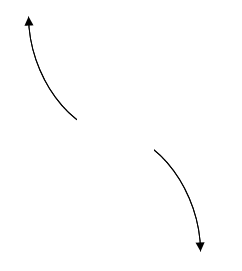
\includegraphics[width=0.3\textwidth]{../Figures/polyEndBehaviorAA.png}
\end{center}\begin{enumerate}[label=\Alph*.]
\begin{multicols}{2}
\item 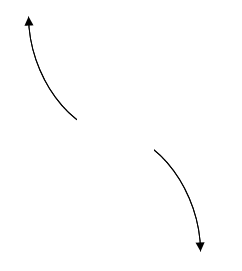
\includegraphics[width = 0.3\textwidth]{../Figures/polyEndBehaviorAA.png}
\item 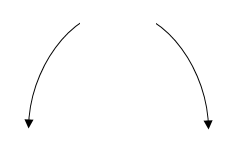
\includegraphics[width = 0.3\textwidth]{../Figures/polyEndBehaviorBA.png}
\item 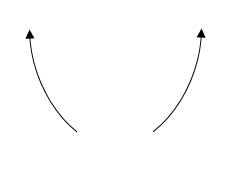
\includegraphics[width = 0.3\textwidth]{../Figures/polyEndBehaviorCA.png}
\item 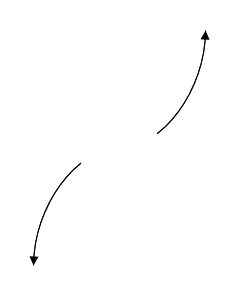
\includegraphics[width = 0.3\textwidth]{../Figures/polyEndBehaviorDA.png}
\end{multicols}\item None of the above.\end{enumerate}
\textbf{General Comment:} Remember that end behavior is determined by the leading coefficient AND whether the \textbf{sum} of the multiplicities is positive or negative.
}
\litem{
Which of the following equations \textit{could} be of the graph presented below?

\begin{center}
    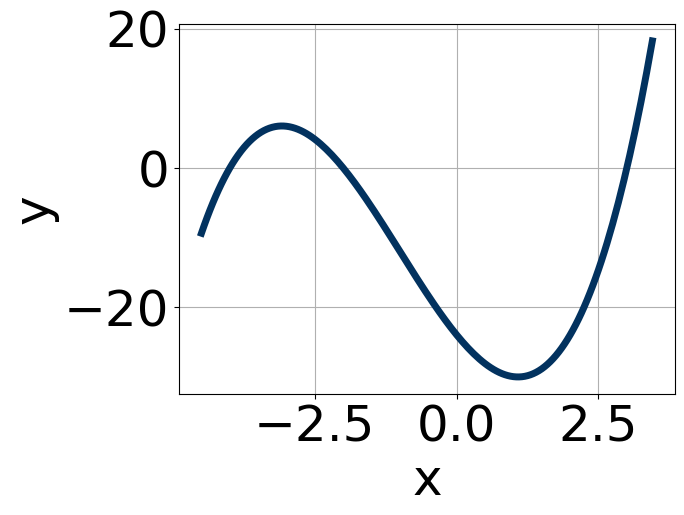
\includegraphics[width=0.5\textwidth]{../Figures/polyGraphToFunctionCopyA.png}
\end{center}



The solution is \( 4x^{9} (x + 3)^{6} (x + 2)^{9} \), which is option C.\begin{enumerate}[label=\Alph*.]
\item \( -15x^{7} (x + 3)^{8} (x + 2)^{5} \)

This corresponds to the leading coefficient being the opposite value than it should be.
\item \( -20x^{4} (x + 3)^{8} (x + 2)^{9} \)

The factor $x$ should have an odd power and the leading coefficient should be the opposite sign.
\item \( 4x^{9} (x + 3)^{6} (x + 2)^{9} \)

* This is the correct option.
\item \( 18x^{7} (x + 3)^{6} (x + 2)^{4} \)

The factor $(x + 2)$ should have an odd power.
\item \( 13x^{7} (x + 3)^{5} (x + 2)^{10} \)

The factor $-3$ should have an even power and the factor $-2$ should have an odd power.
\end{enumerate}

\textbf{General Comment:} General Comments: Draw the x-axis to determine which zeros are touching (and so have even multiplicity) or cross (and have odd multiplicity).
}
\litem{
Which of the following equations \textit{could} be of the graph presented below?

\begin{center}
    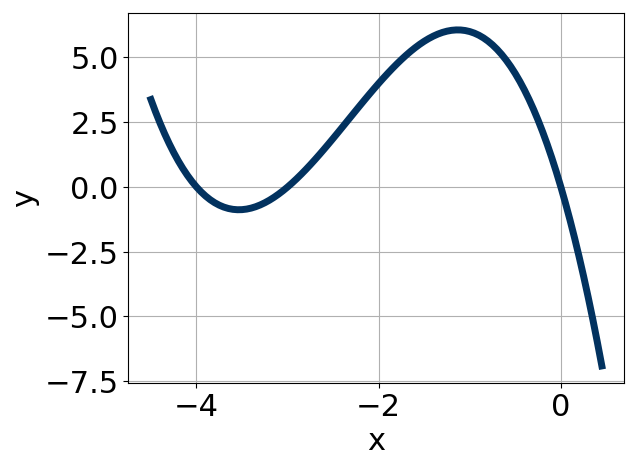
\includegraphics[width=0.5\textwidth]{../Figures/polyGraphToFunctionA.png}
\end{center}



The solution is \( 16x^{5} (x + 1)^{4} (x - 1)^{9} \), which is option A.\begin{enumerate}[label=\Alph*.]
\item \( 16x^{5} (x + 1)^{4} (x - 1)^{9} \)

* This is the correct option.
\item \( 3x^{7} (x + 1)^{6} (x - 1)^{8} \)

The factor $(x - 1)$ should have an odd power.
\item \( -6x^{6} (x + 1)^{10} (x - 1)^{9} \)

The factor $x$ should have an odd power and the leading coefficient should be the opposite sign.
\item \( 6x^{5} (x + 1)^{11} (x - 1)^{10} \)

The factor $-1$ should have an even power and the factor $1$ should have an odd power.
\item \( -4x^{11} (x + 1)^{6} (x - 1)^{11} \)

This corresponds to the leading coefficient being the opposite value than it should be.
\end{enumerate}

\textbf{General Comment:} General Comments: Draw the x-axis to determine which zeros are touching (and so have even multiplicity) or cross (and have odd multiplicity).
}
\litem{
Construct the lowest-degree polynomial given the zeros below. Then, choose the intervals that contain the coefficients of the polynomial in the form $ax^3+bx^2+cx+d$.
\[ -6, \frac{-1}{2}, \text{ and } \frac{-4}{3} \]
The solution is \( 6x^{3} +47 x^{2} +70 x + 24 \), which is option D.\begin{enumerate}[label=\Alph*.]
\item \( a \in [0, 14], b \in [-27, -22], c \in [-65, -57], \text{ and } d \in [-24, -21] \)

$6x^{3} -25 x^{2} -62 x -24$, which corresponds to multiplying out $(x + 1)(2x -2)(3x -3)$.
\item \( a \in [0, 14], b \in [-51, -41], c \in [70, 76], \text{ and } d \in [-24, -21] \)

$6x^{3} -47 x^{2} +70 x -24$, which corresponds to multiplying out $(x -6)(2x -1)(3x -4)$.
\item \( a \in [0, 14], b \in [39, 51], c \in [70, 76], \text{ and } d \in [-24, -21] \)

$6x^{3} +47 x^{2} +70 x -24$, which corresponds to multiplying everything correctly except the constant term.
\item \( a \in [0, 14], b \in [39, 51], c \in [70, 76], \text{ and } d \in [19, 25] \)

* $6x^{3} +47 x^{2} +70 x + 24$, which is the correct option.
\item \( a \in [0, 14], b \in [-36, -27], c \in [-37, -31], \text{ and } d \in [19, 25] \)

$6x^{3} -31 x^{2} -34 x + 24$, which corresponds to multiplying out $(x + 1)(2x + 2)(3x -3)$.
\end{enumerate}

\textbf{General Comment:} To construct the lowest-degree polynomial, you want to multiply out $(x + 6)(2x + 1)(3x + 4)$
}
\litem{
Describe the zero behavior of the zero $x = 3$ of the polynomial below.
\[ f(x) = -2(x + 3)^{7}(x - 3)^{8}(x - 2)^{9}(x + 2)^{11} \]
The solution is the graph below, which is option B.
\begin{center}
    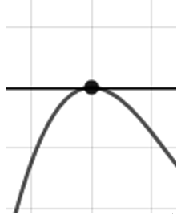
\includegraphics[width=0.3\textwidth]{../Figures/polyZeroBehaviorCopyBA.png}
\end{center}\begin{enumerate}[label=\Alph*.]
\begin{multicols}{2}
\item 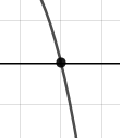
\includegraphics[width = 0.3\textwidth]{../Figures/polyZeroBehaviorCopyAA.png}
\item 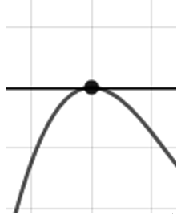
\includegraphics[width = 0.3\textwidth]{../Figures/polyZeroBehaviorCopyBA.png}
\item 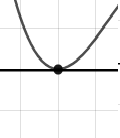
\includegraphics[width = 0.3\textwidth]{../Figures/polyZeroBehaviorCopyCA.png}
\item 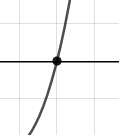
\includegraphics[width = 0.3\textwidth]{../Figures/polyZeroBehaviorCopyDA.png}
\end{multicols}\item None of the above.\end{enumerate}
\textbf{General Comment:} You will need to sketch the entire graph, then zoom in on the zero the question asks about.
}
\litem{
Construct the lowest-degree polynomial given the zeros below. Then, choose the intervals that contain the coefficients of the polynomial in the form $x^3+bx^2+cx+d$.
\[ -4 + 5 i \text{ and } 1 \]
The solution is \( x^{3} +7 x^{2} +33 x -41 \), which is option B.\begin{enumerate}[label=\Alph*.]
\item \( b \in [-1, 6], c \in [-10, -1], \text{ and } d \in [2, 7] \)

$x^{3} + x^{2} -6 x + 5$, which corresponds to multiplying out $(x -5)(x -1)$.
\item \( b \in [4, 11], c \in [32, 39], \text{ and } d \in [-43, -38] \)

* $x^{3} +7 x^{2} +33 x -41$, which is the correct option.
\item \( b \in [-13, -3], c \in [32, 39], \text{ and } d \in [35, 44] \)

$x^{3} -7 x^{2} +33 x + 41$, which corresponds to multiplying out $(x-(-4 + 5 i))(x-(-4 - 5 i))(x + 1)$.
\item \( b \in [-1, 6], c \in [2, 4], \text{ and } d \in [-5, 4] \)

$x^{3} + x^{2} +3 x -4$, which corresponds to multiplying out $(x + 4)(x -1)$.
\item \( \text{None of the above.} \)

This corresponds to making an unanticipated error or not understanding how to use nonreal complex numbers to create the lowest-degree polynomial. If you chose this and are not sure what you did wrong, please contact the coordinator for help.
\end{enumerate}

\textbf{General Comment:} Remember that the conjugate of $a+bi$ is $a-bi$. Since these zeros always come in pairs, we need to multiply out $(x-(-4 + 5 i))(x-(-4 - 5 i))(x-(1))$.
}
\litem{
Describe the zero behavior of the zero $x = -4$ of the polynomial below.
\[ f(x) = -7(x + 4)^{6}(x - 4)^{9}(x - 7)^{5}(x + 7)^{7} \]
The solution is the graph below, which is option B.
\begin{center}
    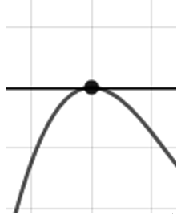
\includegraphics[width=0.3\textwidth]{../Figures/polyZeroBehaviorBA.png}
\end{center}\begin{enumerate}[label=\Alph*.]
\begin{multicols}{2}
\item 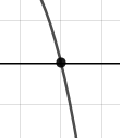
\includegraphics[width = 0.3\textwidth]{../Figures/polyZeroBehaviorAA.png}
\item 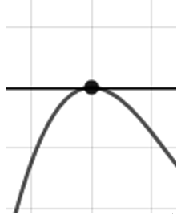
\includegraphics[width = 0.3\textwidth]{../Figures/polyZeroBehaviorBA.png}
\item 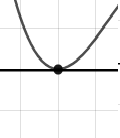
\includegraphics[width = 0.3\textwidth]{../Figures/polyZeroBehaviorCA.png}
\item 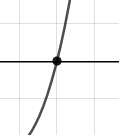
\includegraphics[width = 0.3\textwidth]{../Figures/polyZeroBehaviorDA.png}
\end{multicols}\item None of the above.\end{enumerate}
\textbf{General Comment:} You will need to sketch the entire graph, then zoom in on the zero the question asks about.
}
\end{enumerate}

\end{document}